%%%%%%%%%%%%%%%%%%%%%%%%%%%%%%%%%%%%%%%%%%%%%%%%%
%
%     Chapter 6
%
%%%%%%%%%%%%%%%%%%%%%%%%%%%%%%%%%%%%%%%%%%%%%%%%

\chapter{Performance Evaluation}
\label{six}

In this chapter, we focus on the performance evaluation to show that our LLVM back end could not only match performance with the hand-written library, but also provide a better chance to optimize according to the specific target. We would first validate our vector of $i2^k$ approaches, and then present the performance of some critical Parabix operations via application-level profile.

\section{Vector of $i2^k$ Performance}
In Chapter~\ref{four}, we present different approaches to lower $i1$, $i2$, $i4$ and some $i8$ operations within one SIMD register. In this section, we would validate our approaches by showing the improved run-time performance.

\subsection{Methodology}

Testing small pieces of critical code can be tricky, since the testing overhead can easily overwhelm the critical code and make the result meaningless. Agner Fog provides a test program which uses the Time Stamp Counter for clock cycles and Performance Monitor Counters for instruction count and other related events \cite{agner_testp}. We pick the reciprocal throughput as our measurement and it is measured with a sequence of same instructions where subsequent instructions are independent of the previous ones. In Fog's instruction table, he noted that a typical length of the sequence is 100 instructions of the same type and this sequence should be repeated in a loop if a larger number of instructions is desired.

We did one simple experiment with SIMD XOR ($xorps$) to validate this program. Refer to Figure~\ref{figure:testp_xor}, we measured the performance of executing different number of XOR instructions; they are organized into one for loop and we have checked the assembly code to make sure the XOR operations are not optimized away.

\begin{figure}[ht!]
\centering
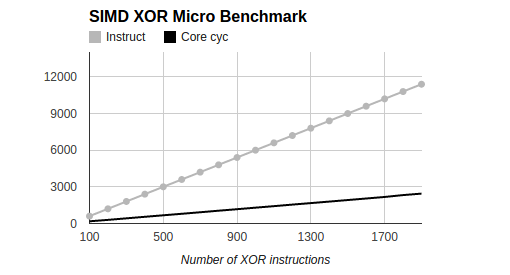
\includegraphics[width=140mm]{draw/testp_xor.png}
\caption[Test Performance with XOR]{Test performance with XOR\@. The dotted line is instruction count and the other line is core CPU cycles.}
\label{figure:testp_xor}
\end{figure}

From the figure, we can see the instruction count and CPU cycles grows linearly with the number of XOR instructions. So we can conclude that Fog's test program can be used to compare two pieces of critical code: the one with more measured CPU cycles is more complex and have more instructions. Note that from the figure, it seems the throughput of $xorps$ is 4, which is different from Intel's document (3 in document). We found this may be related to the compiler optimization on the loop; when we flattened the loop we got the throughput around 2 to 3. In order to eliminate this undesired effect, we would flatten the test code in the following sections.

In the following sections, we would write micro benchmarks with Agner Fog's test program and compare reciprocal throughput between different implementation. Our test machine is X86 64-bit Ubuntu with Intel Haswell, and the detailed configuration can be found in Table~\ref{table:hardware_config}. In order to inline pure IR functions (instead of a function call into one object file), we compile all the test code into LLVM bit code (binary form of LLVM IR) and then link / optimize them together. The default compile flag is to use Intel SSE2 instruction set and on 64-bit OS.

\begin{table}[h]
\centering
\begin{tabular}{|c|c|}
\hline
CPU Name       & Intel(R) Core(TM) i5-4570 CPU \\ \hline
CPU MHz        & 3200                          \\ \hline
FPU            & Yes                           \\ \hline
CPU(s) enabled & 4 cores                       \\ \hline
L1 Cache       & 32 KB D + 32KB I              \\ \hline
L2 Cache       & 256 KB                        \\ \hline
L3 Cache       & 6 MB                          \\ \hline
Memory         & 8GB                           \\ \hline
\end{tabular}
\caption{Hardware Configuration}
\label{table:hardware_config}
\end{table}

\begin{table}[h]
\centering
\begin{tabular}{|c|c|}
\hline
Operating System & Ubuntu (Linux X86-64)         \\ \hline
Compiler         & Clang 3.5-1ubuntu1, GCC 4.8.2 \\ \hline
LLVM             & LLVM 3.4                      \\ \hline
File System      & Ext4                          \\ \hline
\end{tabular}
\caption{Software Configuration}
\label{table:software_config}
\end{table}

\subsection{Performance Against IDISA}
We compare our lowering on pure IR function with IDISA+ Library \cite{hua_idisa} which is written in C++. To test each operation, we generate a sequence of 500 such operations where none them has to wait for the previous one. 100 operations seems not long enough for a stable result. The performance comparison is listed in Figure~\ref{figure:throughput_vector} and Figure~\ref{figure:cpu_cycles_vector}. We can see for $i1$ and $i4$ vectors, IR library has the similar performance with IDISA but it performs better with $i2$ vectors, especially on integer comparison.

The underlying logic for both libraries is the same, but it is implemented in different level. For IDISA library, {\tt simd<2>::ugt} got inline-extended immediately by the compiler front end and its semantics of integer comparison lost ever after, while in the IR library, for the whole life cycle before the instruction selection, {\tt ugt\_2} keeps its semantics and this may help the compiler to optimize. The expansion of {\tt ugt\_2} is delayed until the instruction selection phase, right before machine code generation. We checked that IDISA function {\tt simd<2>::ugt} and IR function {\tt ugt\_2} (whose underlying code is just \verb|icmp ugt <64 x i2> %a, %b|) generated different assembly code.

However, the delay in expansion is not always good. Take multiplication on the $i2$ vector for an example, we can see our IR library has slightly better total CPU cycles, but if we write our instructions sequence with a loop, IDISA library would win (Figure~\ref{figure:loop_vector_i2}). Loop optimization should be responsible for this difference and we did observe some kind of hoisting in the assembly code. Early expansion in IDISA also provides more optimization opportunity to the compiler front end.

Further more, from the reciprocal throughput comparison (Figure~\ref{figure:throughput_vector}), IR library loses a bit on $i1$ vectors but wins most of the cases in $i2$ and $i4$; it may relate to a better instruction selection. IDISA library is generated from a strategy pool based on the number of basic instructions which are treated equally with cost 1. But basic instructions actually have different throughput in the real hardware, and LLVM back end are aware of that, thus selecting better instructions.

\begin{figure}[ht!]
\centering
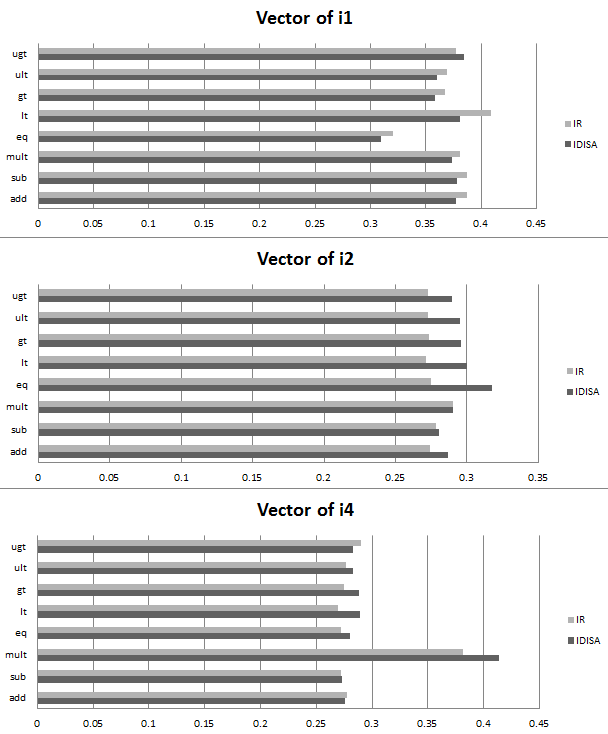
\includegraphics[width=140mm]{draw/reciprocal_throughput_vector.png}
\caption[Reciprocal instruction throughput against IDISA library]{Reciprocal instruction throughput against IDISA library. IR and IDISA share almost identical throughput.}
\label{figure:throughput_vector}
\end{figure}

\begin{figure}[ht!]
\centering
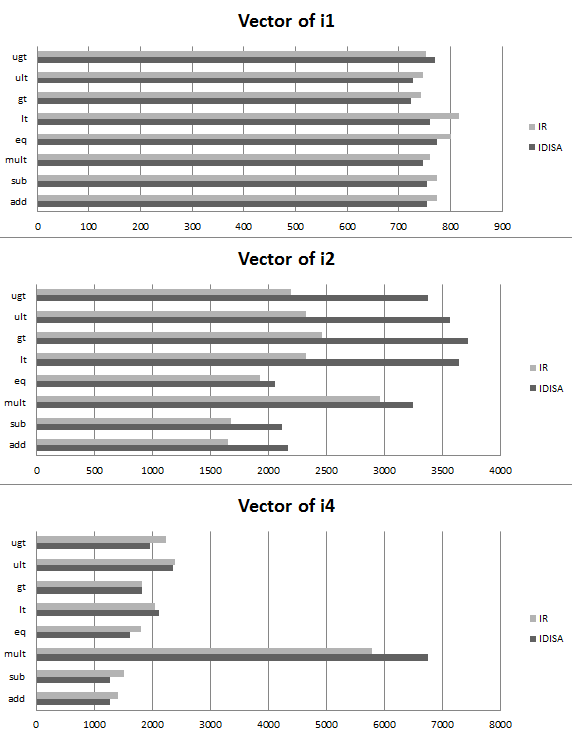
\includegraphics[width=140mm]{draw/cpu_cycles_vector.png}
\caption[Total CPU cycles against IDISA library]{Total CPU cycles against IDISA library; for $i1$ and $i4$ vectors, IR library has the similar performance with IDISA but it performs better with $i2$ vectors, especially on integer comparison.}
\label{figure:cpu_cycles_vector}
\end{figure}

\begin{figure}[ht!]
\centering
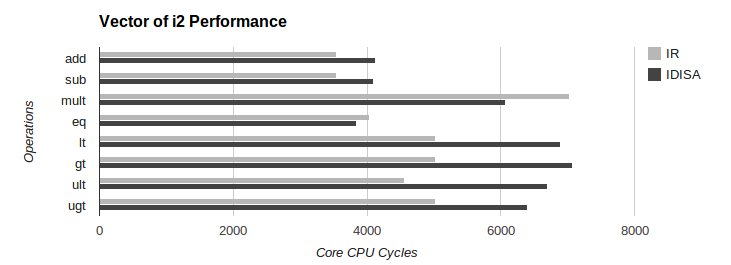
\includegraphics[width=140mm]{draw/loop_vector_i2.png}
\caption[Vector of $i2$ tested in a loop]{The same benchmark for $i2$ vectors with the instruction in a loop. Code in Figure~\ref{figure:cpu_cycles_vector} can be seen as the flattened version of this figure. We find IDISA here wins in the multiplication on $i2$, while IR wins it in Figure~\ref{figure:cpu_cycles_vector}. Loop optimization should be responsible for it.}
\label{figure:loop_vector_i2}
\end{figure}

\subsection{Performance Against LLVM}
We compare our lowering with native LLVM\@. LLVM could not handle $i2$, $i4$ vectors and handle $i1$ vectors slowly. Detailed performance data can be found in Table~\ref{table:vector_perf_LLVM}. We can see that our approach fills the gap of LLVM type system.

\begin{table}[h]
\centering
\begin{tabular}{|c|c|c|c|c|}
\hline
     & $i1$ & $i2$ & $i4$ & $i8$ \\ \hline
add  & 302  & X    & X    & 1\\ \hline
sub  & 310  & X    & X    & 1\\ \hline
mult & X    & X    & X    & 10\\ \hline
eq   & 273  & X    & X    & 1\\ \hline
lt   & X    & X    & X    & 1\\ \hline
gt   & X    & X    & X    & 1\\ \hline
ult  & 349  & X    & X    & 1\\ \hline
ugt  & 290  & X    & X    & 1\\ \hline
\end{tabular}
\caption[Performance against LLVM native support for $i2^k$ vectors]{Performance against LLVM native support of $i2^k$ vectors. `X' means compile error or compile too slowly (longer than 30s), the rest number means the ratio of CPU cycles speed up: add takes 302 times of cycles that our lowering needs. For $i8$, we apply inductive doubling strategy on the multiplication, which explains the 10 times speed up. }
\label{table:vector_perf_LLVM}
\end{table}

\section{Parabix Critical Operations}
In this section, we evaluate our work by replacing Parabix critical operations with the IR library. We first choose transposition and inverse transposition as two representative operations and measure performance in two Parabix applications: XML validator and UTF-8 to UTF-16 transcoder. Note that we did not rewrite the whole application with an IR library, part of the application is still IDISA but some critical operation is replaced. The default compile flag is to use Intel SSE2 instruction set and on 64-bit OS.

\begin{table}[h]
\centering
\begin{tabular}{|c|c|c|c|c|c|}
\hline
        & dew.xml  &  jaw.xml  &  roads-2.gml  &  po.xml  & soap.xml¬ \\\hline
xmlwf0   &  3.93   &    4.364   &   4.553   &   4.891   &   5.18 \\ \hline
xmlwf0 on Haswell   &  3.929   &   4.363   &   4.554   &   4.876   &   5.178 \\ \hline

xmlwf1   &  3.929   &   4.371   &   4.566   &   4.861   &   5.186 \\ \hline
xmlwf1 on Haswell &   3.566   &   3.978   &   4.163   &   4.451   &   4.787 \\ \hline
\end{tabular}
\caption[Performance comparison of XML Validator (xmlwf)]{Performance comparison of XML validator (xmlwf), in a thousand CPU cycles per thousand byte. In the table, xmlwf0 is implemented with full IDISA library and xmlwf1 is a copy of xmlwf0 with the transposition replaced.}
\label{table:xmlwf_perf}
\end{table}

\begin{table}[h]
\centering
\begin{tabular}{|c|c|c|c|c|c|}
\hline
 & dew.xml & jaw.xml & roads-2.gml & po.xml & soap.xml \\ \hline
 U8u16\_0         & 281.46  & 37.11   & 40.06       & 244.94 & 10.2     \\ \hline
 U8u16\_0 Haswell & 272.68  & 34.21   & 39.84       & 242.56 & 10.11    \\ \hline
 U8u16\_1         & 284.17  & 36.71   & 41.65       & 255.57 & 10.6     \\ \hline
 U8u16\_1 Haswell & 267.14  & 34.64   & 38.53       & 237.66 & 9.98     \\ \hline
 \end{tabular}
 \caption[Performance comparison of UTF-8 UTF-16 Transcoder]{Performance comparison of UTF-8 UTF-16 transcoder, in a million CPU cycles. U8u16\_0 is written in IDISA, U8u16\_1 has the transposition and inverse transposition part replaced.}
 \label{table:u8u16_perf}
 \end{table}

Table~\ref{table:xmlwf_perf} shows the performance of the XML Validator. The only difference of xmlwf0 and xmlwf1 is their transposition code, and the one in xmlwf1 is written in pure IR with the byte-pack algorithm. We can see xmlwf0 and xmlwf1 share almost identical performance and it is not for free. LLVM 3.4 cannot handle packing on 16-bit field width very well and we custom lower the shufflevector and generate PACKUS instruction for X86.

Another interesting observation is, when we re-compiled the same code on the Intel Haswell platform, we got almost no improvement for xmlwf0, since the IDISA library linked in is written with SSE2 intrinsic and only SSE2 instructions can be generated; but we got a slightly better performance for xmlwf1, because the IR library is target-independent and LLVM back end knows other instruction sets like SSE3, SSE4 is available on this platform, it generates better code with them.

Similar performance data on UTF-8 to UTF-16 transcoder is listed in Table~\ref{table:u8u16_perf}. U8u16\_0 is written in IDISA and U8u16\_1 has both the transposition and inverse transposition part replaced. We also tried to compile them on the full Haswell, which gave us similar performance benefit.

\subsection{Ideal 3-Stage Transposition on the Intel Haswell}
Intel Haswell architecture introduces PEXT operation which can be used for the ideal 3-stage transposition. We evaluated its performance in Table~\ref{table:PEXT_transposition}. We can see the performance drops with PEXT, but the major reason is that PEXT can only work on $i32$ or $i64$ integer for the current architecture, not the algorithm. As the hardware evolves, we may have PEXT on SIMD registers directly and we can expect a better performance in xmlwf2, may be better than both xmlwf0 and xmlwf1 since 3-stage transposition is proved to be optimal under the IDISA model \cite{inductive_doubling_principle}. Our approach provides a new chance to exploit future hardware benefit without changing the source code.

\begin{table}[h]
\centering
\begin{tabular}{|c|c|c|c|c|c|}
\hline
        & dew.xml  &  jaw.xml  &  roads-2.gml  &  po.xml  & soap.xml¬ \\\hline
xmlwf0 on Haswell   &  3.929   &   4.363   &   4.554   &   4.876   &   5.178 \\ \hline
xmlwf1 on Haswell &   3.566   &   3.978   &   4.163   &   4.451   &   4.787 \\ \hline
xmlwf2 on Haswell & 4.11   &    4.49   &    4.69   &    4.978   &   5.308 \\ \hline
\end{tabular}
\caption[Ideal 3-Stage Transposition with PEXT]{Ideal 3-stage transposition on xmlwf2. Xmlwf1 uses byte-pack algorithm in IR, xmlwf0 uses the same algorithm in IDISA.}
\label{table:PEXT_transposition}
\end{table}

\subsection{Long Stream Addition}
We replaced the internal logic of big integer addition in Chapter~\ref{four} and introduced a new intrinsic: {\tt uadd.with.overflow.carryin}. We would evaluate them in this section by first comparing the long-stream addition algorithm with LLVM's original implementation and then doing some application level profile for the new intrinsic.

We wrote micro benchmarks with Fog's test program and we put 200 independent additions on $i128$ and $i256$. It was tricky to make the test program right, we generated random data for the operands and we carefully inserted the carry-out bit back to the return value so that our long stream addition logic would not be optimized away. In order to be consistent throughout the comparison, we used the same compiler flag for all the runs ({\tt -mavx2} for gcc and {\tt -mattr=+avx2,+bmi2} for LLVM tool chain). The result is listed in Table~\ref{table:lsadd_micro}.

\begin{table}[h]
\centering
\begin{tabular}{|c|c|c|}
\hline
                             & Core CPU Cycles & Instructions \\ \hline
Long stream addition on $i128$ & 2416            & 6552         \\ \hline
LLVM on $i128$                 & 1455            & 4199         \\ \hline
Long stream addition on $i256$ & 2656            & 6959        \\ \hline
LLVM on $i256$                 & 4234            & 9798         \\ \hline
\end{tabular}
\caption{Micro benchmarks for long stream addition against LLVM's original implementation.}
\label{table:lsadd_micro}
\end{table}

Long stream addition does not perform well on $i128$, since there is only two sequential additions involved (1 $addq$ and 1 $adcq$) and parallel computing would not save much but introduce complexity. However, we can see on $i256$ long stream addition has better performance than the sequential one that generates 1 $addq$ and 3 $adcq$. As the width of the operand doubles, the CPU cycles from LLVM increases to the rate of 2.91, while in the long stream addition, the rate is only 1.10. Our algorithm scales better when the width of SIMD registers grows. We could confidently predict that on the Intel AVX512, long stream addition on $i512$ would out-perform the sequential one significantly.

We then show application level profile of `icgrep' which is a tool for regular expression matching with bitwise data parallelism. The internal "add with carry" logic is replaced with one single intrinsic and the performance is plotted in Figure~\ref{figure:lsadd_icgrep}. The performance drops because that version of icgrep works with 128-bit SIMD registers and long stream addition does not work well on $i128$. We could expect better performance on wider SIMD registers.

\begin{figure}[ht!]
\centering
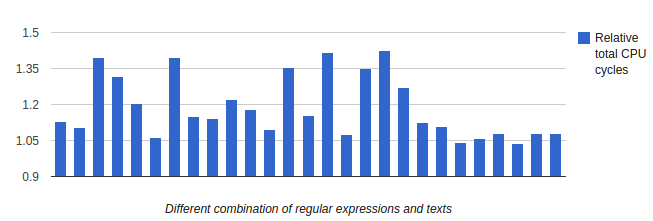
\includegraphics[width=140mm]{draw/lsadd_icgrep.png}
\caption[Performance of icgrep with long stream addition]{Performance of icgrep with long stream addition. This version of icgrep is based on $i128$ so long stream addition actually slows down the performance; but for wider SIMD register, it would get the same performance or even better. For different regular expressions, the portion of "add with carry" code can be different, which explains the difference of the relative cycles across the x axis.}
\label{figure:lsadd_icgrep}
\end{figure}
